\documentclass{standalone}
\usepackage{tikz}
\usetikzlibrary{arrows.meta}

\begin{document}

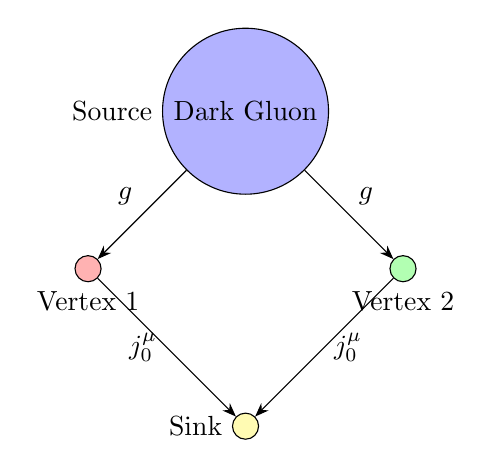
\begin{tikzpicture}[node distance=2cm, >=Stealth]

    % Nodes
    \node (source) [circle, draw, fill=blue!30] at (0,0) {Dark Gluon};
    \node (vertex1) [circle, draw, fill=red!30] at (-2,-2) {};
    \node (vertex2) [circle, draw, fill=green!30] at (2,-2) {};
    \node (sink) [circle, draw, fill=yellow!30] at (0,-4) {};

    % Lines
    \draw[-{Stealth[length=5pt]}] (source) -- node[above left] {$g$} (vertex1);
    \draw[-{Stealth[length=5pt]}] (source) -- node[above right] {$g$} (vertex2);
    \draw[-{Stealth[length=5pt]}] (vertex1) -- node[left] {$j_0^\mu$} (sink);
    \draw[-{Stealth[length=5pt]}] (vertex2) -- node[right] {$j_0^\mu$} (sink);

    % Labels
    \node at (source.west) [left] {Source};
    \node at (vertex1.south) [below] {Vertex 1};
    \node at (vertex2.south) [below] {Vertex 2};
    \node at (sink.west) [left] {Sink};

\end{tikzpicture}

\end{document}